\fancyfoot[C]{G�rel}
\subsection{Python}
Python ist eine interpretierte, hochrangige Programmiersprache, die f�r ihre Einfachheit, Vielseitigkeit und Lesbarkeit bekannt ist. Entwickelt von Guido van Rossum in den sp�ten 1980er Jahren und erstmals ver�ffentlicht im Jahr 1991, hat sich Python zu einer der beliebtesten Programmiersprachen weltweit entwickelt.

\paragraph{Merkmale von Python:}

\begin{itemize}
    \item \textbf{Einfachheit:} Python legt gro�en Wert auf eine einfache und gut lesbare Syntax, die es Entwicklern erm�glicht, 
		Code schnell zu schreiben und zu verstehen. Dies macht Python besonders f�r Anf�nger attraktiv. Diese Art Code zu schreiben wird auch als \textit{Pythonic} beschrieben.
		Diese kann man in jeder Pythonkonsole einsehen, indem man \textit{\textbf{import this}} eingibt.
\begin{figure}[H]
    \centering
    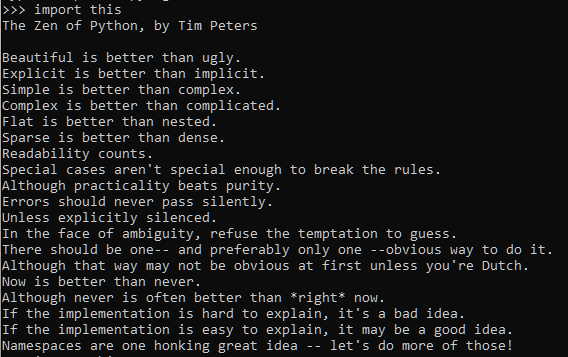
\includegraphics[scale=0.55]{./3_Stand_der_Technik/Abbildungen/pythonic_way.png}
    \caption{Konsole, Pythonic Code}
\end{figure}
    \item \textbf{Vielseitigkeit:} Python wird in einer Vielzahl von Anwendungsbereichen eingesetzt, darunter Webentwicklung, Datenanalyse, k�nstliche Intelligenz, wissenschaftliches Rechnen, Automatisierung, Spieleentwicklung und mehr. Seine Vielseitigkeit und Flexibilit�t machen es zu einer �u�erst n�tzlichen Programmiersprache.
    
    \item \textbf{Interpretation:} Python ist eine interpretierte Sprache, was bedeutet, dass der Code zur Laufzeit von einem Interpreter ausgef�hrt wird, anstatt im Voraus in Maschinencode �bersetzt zu werden. Dies erm�glicht eine schnelle Entwicklung und einfache Fehlerbehebung.
    
    \item \textbf{Plattformunabh�ngigkeit:} Python-Code ist plattformunabh�ngig und l�uft auf verschiedenen Betriebssystemen wie Windows, macOS und Linux. Dies bedeutet, dass Programme, die in Python geschrieben sind, ohne �nderungen auf verschiedenen Plattformen ausgef�hrt werden k�nnen.
    
    \item \textbf{Umfangreiche Standardbibliothek:} Python verf�gt �ber eine umfangreiche Standardbibliothek, die eine Vielzahl von Funktionen und Modulen f�r verschiedene Zwecke bietet. Dadurch wird es einfacher, verschiedene Aufgaben zu erledigen, ohne zus�tzliche Bibliotheken installieren zu m�ssen.
    
    \item \textbf{Dynamische Typisierung:} Python ist dynamisch typisiert, was bedeutet, dass Variablen nicht explizit typisiert werden m�ssen. Der Typ einer Variablen wird zur Laufzeit bestimmt, was die Flexibilit�t des Codes erh�ht.
    
    \item \textbf{Aktive Community:} Python hat eine gro�e und aktive Entwicklergemeinschaft, die st�ndig neue Bibliotheken, Frameworks und Werkzeuge entwickelt. Dieses reichhaltige �kosystem tr�gt dazu bei, dass Python stets relevant und auf dem neuesten Stand der Technik bleibt.
\end{itemize}

